%\documentclass{article}
%\usepackage{graphicx}
%
%\begin{document}
%\section{Introduction}
\setlength{\parindent}{1em}
   
Nowadays any kind of modern production use more and more automatic solutions to achieve new goals. That is why automatic systems use in most cases different robot manipulators. Industries that employ robots in a wide variety of applications are the main customers for robot manufacturers. The manipulator market for research applications, on the other hand, is simply too small for the robot manufacturing industry to develop models specifically for such use. While the hardware and mechanical requirements of developed robots are often similar for both industry and research, scientific software requirements are quite different and even contradictory in many aspects. The goal of scientists is to try to gain as much control over the robot as possible, whereas industries seek safe and easy operational interfaces. 

Some of the pioneering companies in the Industrial robotics market are ABB Ltd., Fanuc Corp., Yaskawa Electric Corp., Apex Automation and Robotics, Mistubishi Electric Corp. and KUKA AG. We had the opportunity to work with the latter, KUKA AG, on their model KR6 R900 sixx.
%Over the course of our final year, this project helped increase our knowledge, not only on the main topic, milling and visual servoing, but also on the KUKA platform itself, which is considered an advanced platform widely used in today’s industries. 
\begin{figure}[H]
    \centering
    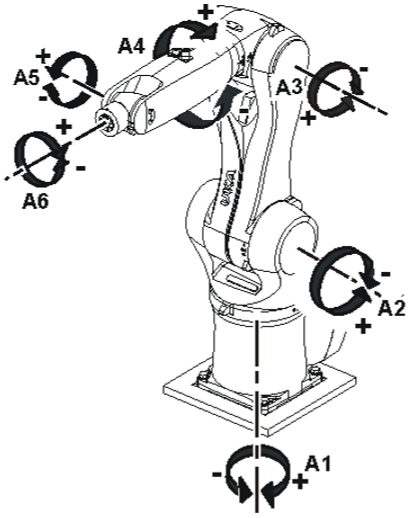
\includegraphics[scale=0.40]{figures/specs6}
     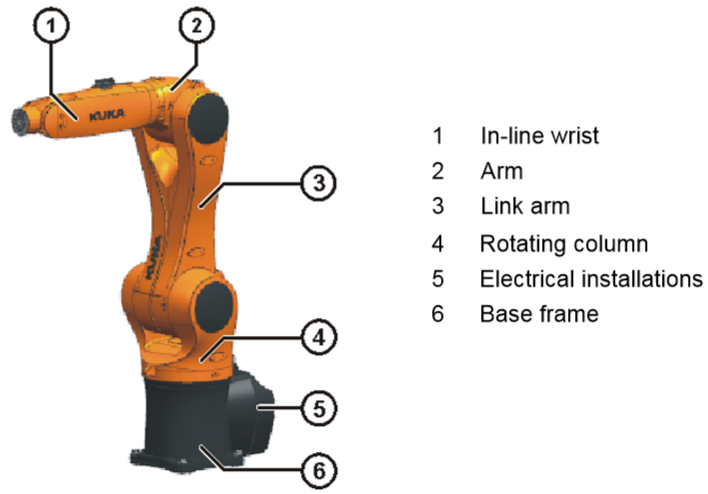
\includegraphics[scale=0.45]{figures/specsc}
    \caption{KUKA KR6 R900 sixx robotic manipulator}
\end{figure}

This robot can carry up to \textbf{6}kg of payload, and reach any point in range of \textbf{900}mm away from its base with \textbf{six} degrees of freedom posing. The robot model name indicates these specifications "KR\textbf{6} R\textbf{900} \textbf{sixx}". It's part of the \textbf{KR AGILUS} series, which includes many other robot varieties for the payload, maximum reach, and the degrees of freedom. 

This robot was purchased three years before starting this project, but no one had commissioned the robot nor installed it properly. We were the first group to use this robot.
 
Before using any industry level robot arm, it first needed to be fixed of a proper- vibration free base setting, then calibrated to get its encoders to work properly. We needed to go through the manuals to learn how to fix, master (calibrate),and program the robot. The design and manufacturing of a base to support the robot during heavy duty operation included performing mathematical calculations based on the robot’s weight and forces to obtain the optimal dimensions and weight for the base, besides performing CAD studies on the manipulator’s body to support the results of the mathematical analysis.

We'd done lots of experiments to learn the syntax of the KRL (KUKA Robot Language). Too much time had been consumed due to lack of resources. We'd found that in addition to robots’ ability to perform several tasks; by adding the desired end-effector and designing the corresponding programming tool, they offer more variations of one task offered by a conventional machine. We'd decided that our project would include two more phases:  \textbf{Implementation of an industrial application}- through developing post-processing tools to convert any conventional G-Code into KUKA Robot Language (KRL) and use the robot for 2D drawing and 3D milling, and \textbf{ Implementation of two research applications} related to visual servoing- through using Kinect interfacing on ROS to guide the robot with hand gestures and provide human-safe operating zone where the robot stops when a human approaches, which made possible after developing an API to control the robot directly from any PC.	
 
%The milling process witnessed vast development since the early milling machines, known as mills, followed by CNC milling machines and all the way to milling robots. The latter, represented in KUKA robots in our project, can be compared to CNC machines in terms of introducing a computer-based control method, however, milling robots offers more advantages than the conventional CNC machines. One of these advantages is flexibility, because as the needs of manufacturing evolve; robots are proving to be nimble adjusters. 
	
\bigskip
	
%	In addition to robots’ ability to perform several tasks; by adding the desired end effector and designing the corresponding programming tool, they offer more variations of one task offered by a conventional machine. To verify this we can compare CNC milling machines and milling robots. 

%CNC machines offer two-dimensional milling operations, moving either horizontally or vertically with fixed workpiece, resulting in a defined scope of products and processes. Milling robots on the other hand, are able to perform milling in up to six axes, providing rotation and movement in multiple directions. This flexibility can further be improved by providing a movable workpiece fixation, increasing the motion axes to nine.
	
We decided to use the robot in milling, because robots offer ease of use through programming, flexibility, speed, precision, cost reduction, repeatability and some of these robots even offer different mounting choices, as they could be mounted on ceilings and walls not just floors.

We first made a 2D-level post-processor extension on Inkscape software, that automatically converts any drawings and text into KRL code files. These files were transferred to the robot, and when executed, the robot made the exact required task. We'd attached a pen, simulating a laser beam to demonstrate this through drawing. Later, we were able to develop 3D post-processing tools for the 3D milling process. 
%all of this contributed to the current status of milling operations; in terms of final finishing, level of details obtained, rate of production and future possibilities for development. 

	
	
%	The project is inspired by the aforementioned development in the industrial sector. The scope of the project can be summarized in the following three points; firstly, the commissioning and operation of the KUKA KR6 R900 sixx robotic manipulator, which included the installation of the related software and creating a network that facilitates communications with the robot. In addition to software commissioning, hands-on experience with the KUKA robot language (KRL) platform was achieved through learning the basic and advanced forms of KRL, which later helped in the development of software tools that facilitates the main objective of the project; the milling process. 
	
%\smallskip	
%	Secondly, the design and manufacturing of a base to support the robot during heavy duty operation, this included performing mathematical calculations based on the robot’s weight and forces to obtain the optimal dimensions and weight for the base, besides performing CAD studies on the manipulator’s body to support the results of the mathematical analysis. 
	
\medskip
	
	%82Finally, the development of various software tools to achieve the purposes of remotely controlling the robot and milling. These tools include an Inkscape extension for converting 2D G-code to KRL, directly using sketches from Inkscape, an independent toolkit for converting 3 axis G-code to KRL. In addition to Python tools; one Python class for reading and writing system variables, and a Python library for controlling the arm motions from pc. The development also included editing openni\_tracker for publishing uncalibrated person's depth and creating ROS nodes for safety operation distance and visual servoing (hand guiding) for the robot.
	
	%Initially, the project scope was limited to the milling process in addition to minor ideas in the smart development of the workspace, however, over the course of the semester we encountered many problems that required extended research in all the previously mentioned aspects, which eventually led to broadening the scope of the project to include these development tools, both relevant and irr*98 elevant to milling. 

	%\section{References}
	%\begin{enumerate}
%		\item http://www.mmsonline.com/articles/a-new-milling-101-what-milling-is-then-and-now-plus-a-glossary-of-milling-terms
		%\item http://www.sickinsight-online.com/safety-and-more-sick-provides-protection-and-navigation-data-for-kukas-kmr-iiwa/ 
		%\item http://medicaldesign.com/contract-manufacturing/modern-cnc-machining-prescription-product-development 
		%\item http://articles.sae.org/11272/ 
		%\item https://en.wikipedia.org/wiki/Multiaxis\_machining 
		%\item https://en.wikipedia.org/wiki/Milling\_(machining) 	
	%\end{enumerate}
	

%\end{document}